\documentclass{article}

\usepackage{verbatim}
\usepackage{minted}
\usepackage{graphicx}

\title{Langages synchrones : TP2}

% A rendre le 04/11
% Metronome: 1,2,3,6
% Arbitre McMillan: 1,2
% Extensions: Q1 (non determinism), Q2 (asynchronisme)

%ssh 3367424@ssh.ufr-info-p6.jussieu.fr

\author{I\~{n}igo Mediavilla \& Pierrick Couderc}

\begin{document}

\maketitle

\section{Métronome}

\subsection{Noeud Lustre}

\begin{verbatim}
node metronome (reset : bool; delay : int) 
     returns (tic, tac : bool);
  var n, hz : int;
      state, first, tmp: bool;
let
    hz = 0 -> if reset then delay - 1 else pre hz;
    n = 0 -> if reset then delay
             else if pre n = 0 and first then hz
             else (pre n) - 1;
    first = false -> reset or pre first;
    state = n = 0 and first;

    tmp = true -> if state then not pre tmp else pre tmp;
    
    tic = if state then tmp else false;
    tac = if state then not tmp else false;
tel
\end{verbatim}


In the figure~\ref{trace-metronome-1} we can see how the given code
emulates the behaviour of the metronome. In the step 6, we set a
delay of 1 and we verify that the metronome emits tics and tacs
alternatively. In the step 13 we modify the delay to 5 and we not
only see how this delay is respected but also how the next signal
emitted is not tic but tac, since the last sinal emmited with delay
1 was tic.

\subsection{Automaton}

The code for C for the metronome that is generated with the commands
lus2oc and poc is shown in figure~\ref{metronome-0}.

\begin{figure}[ht]

\begin{minted}[mathescape,
               linenos,
               numbersep=5pt,
               gobble=2,
               frame=lines,
               framesep=2mm]{c}
  switch(ctx->current_state){
   case 0:
      ctx->_V5 = (ctx->_V3? _false : (ctx->_V1 || ctx->_V5));
      ctx->_V6 = (ctx->_V3? 0 : (ctx->_V1? (ctx->_V2 - 1) : ctx->_V6));
      ctx->_V4 = (ctx->_V3? 0 : (ctx->_V1? ctx->_V2 : (((ctx->_V4 == 0) &&
   ctx->_V5)? ctx->_V6 : (ctx->_V4 - 1))));
      ctx->_V10 = ((ctx->_V4 == 0) && ctx->_V5);
      ctx->_V7 = (ctx->_V3? _true : (ctx->_V10? (!ctx->_V7) : ctx->_V7));
      ctx->_V3 = _false;
      ctx->_V8 = (ctx->_V10? ctx->_V7 : _false);
      metronome_O_tic(ctx->client_data, ctx->_V8);
      ctx->_V9 = (ctx->_V10? (!ctx->_V7) : _false);
      metronome_O_tac(ctx->client_data, ctx->_V9);
      ctx->current_state = 0; break;
   break;
   } /* END SWITCH */
\end{minted}
\label{metronome-0}
\caption{Code C generated with with lus2oc -0 and poc}
\end{figure}

The correspondance of the variables in the C code with
respect to the code in lustre is the following:

\begin{itemize}
\item V1 = reset
\item V2 = delay
\item V3 = initial state = false
\item V4 = n              
\item V5 =          
\item V6 = hz
\item V7 = tmp               
\item V8 = tic  
\item V9 = tac
\item V10 = state
\end{itemize}

And thus the corresponding automaton for the C code is shown
in figure~\ref{automaton-0}

\begin{figure}[!ht]
\begin{center}
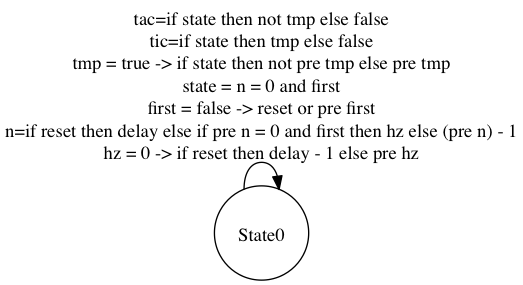
\includegraphics[width=0.8\textwidth, natwidth=610,natheight=642] {automaton-0.png}
\end{center}
\label{automaton-0}
\caption{Automaton without unfolding}
\end{figure}

If we generate the automaton with the option -2, the automaton
is unfolded so the only state that we had for the option -0, is
converted into 4 states. As demonstrated by figure~\ref{automaton-2}
the automaton is unfolded based on the values of the signals \emph{reset}
and \emph{state}.

\begin{figure}[!ht]
\label{automaton-2}
\caption{Automaton with unfolding}
\begin{center}
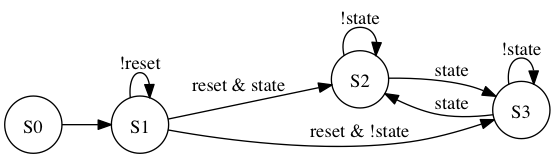
\includegraphics[width=0.8\textwidth, natwidth=610,natheight=642]{automaton-2.png}
\end{center}
\end{figure}

%\begin{figure}
%\label{trace-metronome-1}
%\caption{Execution of the metronome}
%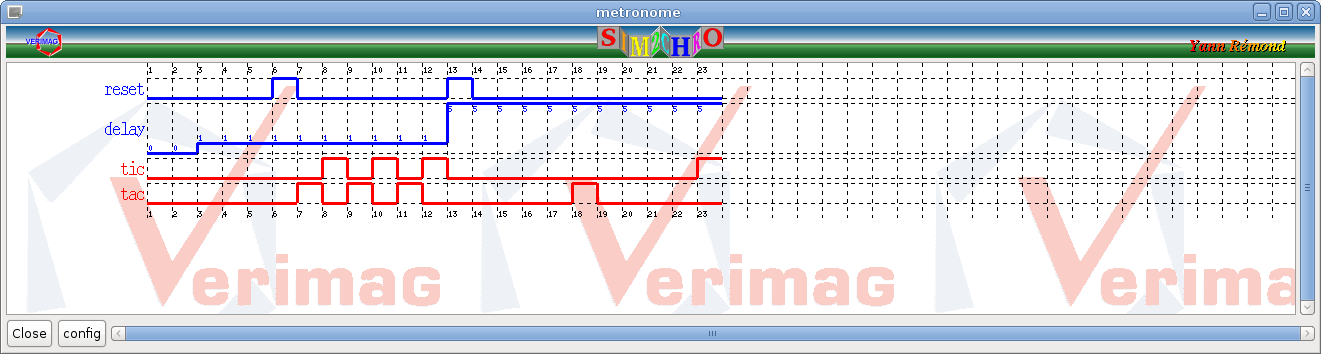
\includegraphics [scale=0.4]{metronome_1.png}
%\end{figure}
\end{document}
